\documentclass[a4paper,draft]{article}
\usepackage{scrextend}
%% for stopping floats
\usepackage{placeins}

%% Language and font encodings
\usepackage[english]{babel}
\usepackage[utf8x]{inputenc}
\usepackage[T1]{fontenc}
\usepackage[normalem]{ulem}
\useunder{\uline}{\ul}{}

%% Sets page size and margins
\usepackage[a4paper,top=3cm,bottom=2cm,left=3cm,right=3cm,marginparwidth=1.75cm,headheight=55pt]{geometry}

%% Useful packages
\usepackage{amsmath}
\usepackage{graphicx}

%% For todo 
\usepackage[pdftex,dvipsnames]{xcolor}  % Coloured text etc.
\usepackage[colorlinks=true, allcolors=blue]{hyperref}
\usepackage{xargs}                      % Use more than one optional parameter in a new commands
\usepackage[obeyDraft,colorinlistoftodos,prependcaption,textsize=tiny]{todonotes}
\newcommandx{\unsure}[2][1=]{\todo[linecolor=red,backgroundcolor=red!25,bordercolor=red,#1]{#2}}
\newcommandx{\change}[2][1=]{\todo[linecolor=blue,backgroundcolor=blue!25,bordercolor=blue,#1]{#2}}
\newcommandx{\info}[2][1=]{\todo[linecolor=OliveGreen,backgroundcolor=OliveGreen!25,bordercolor=OliveGreen,#1]{#2}}
\newcommandx{\improvement}[2][1=]{\todo[linecolor=Plum,backgroundcolor=Plum!25,bordercolor=Plum,#1]{#2}}
\newcommandx{\thiswillnotshow}[2][1=]{\todo[disable,#1]{#2}}
%% todo ends

%% for strike out, normalem
\usepackage[normalem]{ulem}
%% strike out ends

%% for line break in colorbox
\usepackage[]{tcolorbox}


%% no float table
\usepackage{float}
\restylefloat{table}

%% for header
%\usepackage{fancyhdr}

%%\usepackage[headheight=55pt]{geometry}

%\renewcommand{\headrulewidth}{2pt}
%\fancypagestyle{plain}{%
%  \fancyhead[L]{
%    \begin{tabular}{ll}
%%      \begin{tabular}[t]{c}
%        %\includegraphics[scale=0.3]{beeduck}%
%      \end{tabular} &
%      \begin{tabular}[b]{l}
%        \unsure{unsure} \change{change} \info{info} \improvement{improve}
%        Head of Department: The Bee Duck\tabularnewline
%        Vice chairmen: The Duck Bee\tabularnewline
%      \end{tabular}
%    \end{tabular}   
%  }%
%}

\pagestyle{plain}
%% end header

% for extra sub section
\usepackage{titlesec}
\titleclass{\subsubsubsection}{straight}[\subsection]

\newcounter{subsubsubsection}[subsubsection]
\renewcommand\thesubsubsubsection{\thesubsubsection.\arabic{subsubsubsection}}
\renewcommand\theparagraph{\thesubsubsubsection.\arabic{paragraph}} % optional; useful if paragraphs are to be numbered

\titleformat{\subsubsubsection}
  {\normalfont\normalsize\bfseries}{\thesubsubsubsection}{1em}{}
\titlespacing*{\subsubsubsection}
{0pt}{3.25ex plus 1ex minus .2ex}{1.5ex plus .2ex}

\makeatletter
\renewcommand\paragraph{\@startsection{paragraph}{5}{\z@}%
  {3.25ex \@plus1ex \@minus.2ex}%
  {-1em}%
  {\normalfont\normalsize\bfseries}}
\renewcommand\subparagraph{\@startsection{subparagraph}{6}{\parindent}%
  {3.25ex \@plus1ex \@minus .2ex}%
  {-1em}%
  {\normalfont\normalsize\bfseries}}
\def\toclevel@subsubsubsection{4}
\def\toclevel@paragraph{5}
\def\toclevel@paragraph{6}
\def\l@subsubsubsection{\@dottedtocline{4}{7em}{4em}}
\def\l@paragraph{\@dottedtocline{5}{10em}{5em}}
\def\l@subparagraph{\@dottedtocline{6}{14em}{6em}}
\makeatother

\setcounter{secnumdepth}{4}
\setcounter{tocdepth}{4}

% end e-s section

%% 	mind map 
%%\usepackage{epsfig}
\usepackage{tikz}
\usetikzlibrary{mindmap,backgrounds}
%% end mind map


\newcommand{\blap}[1]{\smash[b]{\begin{tabular}[t]{@{}c@{}}#1\end{tabular}}}

\title{Scene Analysis based Bluetooth Low Energy Indoor Positioning Methods\\ \textnormal{Master's Thesis Proposal} \textnormal{v0.4}}
\author{Srikanth Gadicherla}

\begin{document}
\maketitle
\renewcommand{\arraystretch}{1.5}
\thiswillnotshow{ \section{Abstract}
The thesis aims at getting a proof of concept for solutions to the \textbf{hybrid bluetooth low energy indoor positioning}(BLE-IP) along with \textbf{automatic node location identification}(ANOLI). ANOLI is mainly aimed during the calibration phase which gives out the locations of the bluetooth low energy(BLE) beacons. The BLE beacons are present inside the luminaires. The luminaires might either be installed in the ceiling or tethered to it. The location of BLE beacons determined using ANOLI and received signal strength indicator(RSSI) together are used in the BLE-IP task. The factors influencing the RSSI values is also studied and based on the target environment and accuracy the model is decided.  Simple applications like asset tracking is also implemented. }


\section{Goal of the thesis: Description}
\begin{enumerate}
\item \textbf{Automatic Node Location Identification(ANOLI):}
\begin{addmargin}[0em]{0em}% 1em left, 2em right
This task involves finding the locations of the beacons intelligently. Currently, Active Aheads, can read the RSSI values from all the other beacons, so, we need to employ an Machine Learning method for creating a topology of sensors. This task can also be named Self Organizing Sensor Network. The feasibility study is yet to be done but the main idea here is that combining the data from all the sensors and create a topology of sensors and get metadata out of it. This metadata would include to which cluster the particular sensor would belong to, clusters relative position to some landmark location, etc. \cite{raivisto} \\
So, we will have 2 weeks after the commissioning of the luminaires. 

\end{addmargin}

\item \textbf{Develop an algorithm for Bluetooth Low Energy Indoor Positioning(BLE-IP):}
\begin{addmargin}[0em]{0em}% 1em left, 2em right
In this task we want to find the position of a subject given the received signal strength indicator(RSSI) from the BLE beacons. This method would also make use of the information gained during the previous task. So, the idea here is that the metadata is loaded in to the mobile application, and when it starts reading the signal and it will relate the particular MAC(media access control) address to the topology and be used in the memory and non-memory methods. This metadata could also include the current sensor data, and the plan is to integrate as much data as possible for getting better accuracy. There is also conscious effort to make the application have less/no dependency on the internet. \\
The first task would be to understand the different biases via experiments so as to build a broad model which could be used in variety of environments. Then the different methods are deployed to check the accuracy based on that.\\

\textbf{Challenges:}
Need to deal with the different sampling frequencies of different AP's(BLE, WIFI) or smart-phone sensors in the algorithm [Check balzer82 github page or check Torres-Sospedra et al, 2.3, Para 2]
\end{addmargin}
\thiswillnotshow{
\item \textbf{Other tasks}:
\begin{enumerate}
\item \textbf{Applications:}
\begin{itemize}
\item \textbf{Asset tracking} could be accomplished. It includes a BLE device which sends out an advertisement signal which is read by the BLE devices in the mesh network for tracking its location. This is an inspiration\unsure{check this}  from Active Bat Localization System which uses Ultrasound\cite{hightower} \change{??} rather than bluetooth. Here, the bat is indoor mobile tags, similar to an asset.  
\end{itemize}
\item  \textbf{Pattern Recognition}: Another task would be to use the positioning data with other sensor data from smartphone over a period of time to learn spatial and temporal patterns\cite{he}. \info{check the IP\_LiFs\_MDS slides}
\
(Fingerprinting, radio map,..)
\end{enumerate}}

\end{enumerate}

\section{Introduction} \label{intro}
Indoor positioning(IP) is moving towards becoming ubiquitous and fulfilling the goal of Internet of Things(IoT) and Artificial Intelligence(AI) of Location Aware services\improvement{[cite here]}.  The explosion of usage of smartphones in the last decade has also enabled an exponential growth of this field. IP mainly leverages the sensor hub in smartphones like accelerometer, gyroscope, barometer, proximity, thermometer, pedometer, magnetic sensor, etc and wireless technologies like bluetooth and WiFi for accurately solving this problem. Signals of opportunities like magnetic field, pressure, light and sound intensity, Global Navigation Satellite System [Torres-Sospedra et al, A realistic evaluation of indoor positioning systems based on Wi-Fi fingerprinting, 2017], mobile network \cite{99} and frequency modulation(FM)\cite{98} signals have also been used which don't incur any additional infrastructure costs.  IP also gets impetus from interrelated fields like geo-location, augmented reality, natural user interface, gaming, man-machine interaction, and 3D mapping.

\vspace{3mm}
The need for indoor positioning arose because the traditional Global Positioning System(GPS) fares badly indoors due to signals attenuation and scattering caused by roofs and walls. This leads to higher uncertainty in estimation of location which sometimes spans across multiple rooms sabotaging the whole positioning problem. \improvement{put it to some other good place} Usage of indoor positioning(IP) can also be reasoned by following reasons \change{change the adjective here, not quite intuitive} condition, \unsure{right word?} convenience and commercialization. Condition in the sense people tend to stay indoors 90\% of the time according to Environment Protection Agency(EPA) \cite{geospatial}. Convenience as it can be used for locating rooms and tracking assets. Commercialization, in case of malls, groceries stores, can be used to send out discount coupons, personalized recommender engines. The positioning data could also be used to optimize the resource flow in hospitals or warehouse to minimize the operation cost\cite{max}.

\vspace{3mm}
Formally, the estimation of location of mobile unit(MU) using wireless technologies is called location sensing, geo-location, position location or radio-location\cite{liu}. The conventional GPS suffer with problems like building occlusion, multipath effect \cite{fang} and signal attenuation \cite{geospatial} \improvement{cite classic text book} indoors, and hence many other technologies have been advocated. \improvement{improve it} Even though the GPS technology can be improved using the GPS repeaters, the solution is not scalable and would require costly infrastructure. The new technologies for positioning include Assisted GPS, \thiswillnotshow{GPS + cellular mobile tower signal} Bluetooth Low Energy(BLE), MEMS sensors, LED, WiFi, Magnetic anomalies \unsure{is it fine if I use abbreviations directly} or methods used in conjunction with each other \cite{geospatial}. 

IP has been solved using the triangulation techniques like lateration with  time of arrival(TOA), time difference of arrival(TDOA), angle of arrival(AOA), received signal strength(RSS) or fingerprinting based scene analysis methods like decision based probabilistic method, k-Nearest Neighbour(k-NN), artificial neural networks(ANN) or proximity based methods\cite{liu} and Gaussian processes with latent variable models\cite{ferris}. For the rest of the article, we use beacons and nodes interchangeably. 
 \\

\info[inline]{ 
 1. AOA needs at least two known sources. 2. i-locate, open geo-data. \url{http://www.i-locate.eu/pilot-sites/}. 3. Before the advent of  bluetooth low energy(BLE) beacons, the indoor positioning was ....}

\subsection{Setup}
The BLE beacons are part intelligent luminaires are densely packed, the nodes can read the signal strengths from neighboring nodes. Generally, a location estimation task involves two hardware devices, one transmitting the signal and other receiving it\cite{liu}. Here, the transmitting device is bluetooth low energy chip(or WiFi router?) installed in Active Aheads. The other sensor data (there is no infrastructure for getting these data as of now),  follow-strength values is planned to be downloaded once and updated biweekly or monthly. The Active Aheads are part of a mesh network.
\section{Related Work}
In this chapter, we discuss the existing methods and state of the art.
\info[inline]{But it is essential to understand that the method and level of accuracy required is mostly application dependent.}
\improvement{add what each section does}

\subsection{Statistical Data analysis of RSSI values}
The analysis of the received signal strength values could lead to better understanding of features and patterns for a particular fingerprint \thiswillnotshow{from which an appropriate model could be used}. Previously studies were based on RSSI and were mainly directed towards communication technologies rather than positioning systems, hence a clearer knowledge and analysis of this would lead to better modeling and design of positioning systems\cite{kaemar}. The RSSI values suffer attenuation due to reflection, refraction, multipath effect, number of people, indoor environment[Hightower et al, Location Sensing Techniques, A Technical report, 2001], orientation of phones\improvement{(using the compass), for experiments} and quality of BLE chip in the MU's. One more  \cite{deluca}. There's always a trade-off between number of access points and signal interference, but even with the increase in nodes there is an irreducible error due to power measurement noise and quantization, hence can't be reduced below a certain value. Its also because of movement of people and MUs, there is time-correlated fluctuation of RSSI, which sometimes severely affect the performance of positioning solutions\cite{kaemar}.

The different ways of measuring the RSSI values, one, the measurement has standard deviation of 2.5 dBm while the phone was held still.\improvement{add the rotating and cardinal directions.} The presence of human widely varied the signal strength values \improvement{how much and cite it}. But according to \cite{kaemar}, the consideration phone orientation didn't improve the accuracy much. 

\subsubsection{Preprocessing and Manipulation of RSSI values}
From \cite{honkavirta}, for multiple measurements recorded at a single time step, generally the mean of all measurements is taken into consideration.

\noindent
\subsubsection{How hardware effects the measurement of RSSI values?}
The effects of MU's hardware can be useful in estimating the measurement noise and modeling the same, it was seen that variation was 5dBm across different devices.\cite{deluca}

\subsubsection{Modeling based on variation in RSSI values}
The probability distribution of RSSI is a function of location of time as the indoor setting is extremely convoluted. This leads to bimodality and asymmetric nature, hence modeling a better data model is daunting task. The skewness of the RSSI values depends on the distance and presence of obstacles leading to either left or right skewness, or sometimes it could also be symmetric. The left-skewness of the RSSI which is due to large variation of smaller values than information rich higher values values and these are modeled as log-normal distribution [Honkavirta et al, 2009]. It is also approximated using Gaussian distribution or exponential distribution. The limitation of smartphone in registering low signal values and quantization also exacerbates this problem. 

\subsection{RSS based Localization Algorithms}
\subsubsection{Triangulation} 

Triangulation includes methods like Lateration and Angulation, which are described. This method requires estimates from at least three different known sources.

\begin{itemize}
\item \textbf{Lateration}
Lateration\cite{liu} accomplishes the position estimation problem by measuring the distances from known reference points, hence it is also called \textbf{range measurement technique}. Most of the times distance is indirectly measured via either received signal strength(RSS), time of arrival(TOA) or time difference of arrival(TDOA). TOA works on the principle that time and distance positively correlate with each other and given one other can be estimated. But care has to be taken that transmitter and receiver are properly synchronized. TDOA works on time difference of time taken by different measurement devices for receiving the signal. Signal attenuation based models(RSS) try to learn the path loss component due to propagation as the signal in indoor setting is degraded due to multipath fading. Other methods include roundtrip-time-of-flight(RTOF) and received signal phase method. These methods could be used in conjunction with each other to better the accuracy.

\noindent
\textbf{Drawbacks in Lateration:} Multi path and lack of line of sight complicates the problem in TOA, TDOA and Signal attenuation based methods. The location of nodes should be known beforehand.

\item \textbf{Angulation} : The location estimate is found out using finding angle of the target along some fixed reference with at least two known nodes.

\noindent
\textbf{Drawbacks in Angulation:} Need expensive, large and complicated hardware equipment. This method also suffers from multipath reflection.
\end{itemize}

\subsubsection{Static Scene Analysis(Fingerprinting)}

Scene Analysis involves inferring based on features already recorded for a particular location and static scene analysis looks up into a pre-recorded dataset which maps locations with it features\cite{hightower}. Hence, it is also called Fingerprinting as it aims at creating unique feature map based on location dependent measurements. This method involves matching the measured signal with location-dependent ground truth signal. To obtain the ground truth signal, some pre-defined points called \textbf{reference points} \improvement{my defintion of radio-map} are selected and RSSI measurements are recorded from all the available nodes. These ground truth measurements/pre-recorded dataset with location tag is called \textbf{reference table}. The reference table can be used to create a radio-map unlike \cite{honkavirta}.\unsure{check this out, } This can be done either with a simple pathloss interpolation or Gaussian process regression.  This reference table in conjunction with test measurements can be used with deterministic or probabilistic methods for obtaining the location estimate\cite{liu}. \cite{mazzullah} calls this method as template matching algorithm, with reference table and test measurements data called as offline and online data respectively. \cite{honkavirta} calls the offline phase as calibration phase. These data can also be used in sequential Monte Carlo methods like Bayesian Filters (Grid Filter, Kalman Filter, Extended Kalman Filter, Unscented Kalman Filter, Particle Filter) in conjunction with Gaussian Processes both simple and Latent Variable Models or k-Nearest Neighbors.

\vspace{3mm}
\noindent \textbf{For the construction of radio map,} most of the authors have recorded the measurements keeping their MU's still but \cite{honkavirta} have rotated at the given position while recording the measurements to minimize the orientation bias and at the same time they have increased the calibration time to maximize the reliability of the measured data\cite{??}. These have also been recorded in the four different cardinal directions\cite{richter}.This goes in-line with \cite{??} which advocates more the samples better the fingerprint during calibration phase. \cite{honkavirta} splits the floor into cells and assumes the likelihood to be constant inside the cell and in addition also uses methods like histogram and histogram comparison.
\noindent

Advantages of scene analysis over other methods is that it doesn't require any additional information about the devices in contrast to triangulation methods like time-of-flight, time-difference of flight where extra synchronization is essential and in conjunction with GP's it is scalable\cite{hightower}.

\textbf{Few observation about Calibration phase}: Calibration time more than 10 secs doesn't help. And also increasing in AP's doesn't increase accuracy beyond some point. The Grid size for calibration depends on the floor plan and location of the access points. 

\noindent
In simple Gaussian process(GP) model, we use simple GP regression to predict the RSSI values at the other locations and then use a simple Gaussian model for evaluating the likelihood model. One major advantage of using semi-parametric model is that with enough evidence the non-parametric counterpart can override the parametric one\cite{richter}.



\improvement{what is the learning when we are using k-NN?} \\



\textbf{What methods have been used?}
[Mazzullah Khan et al,2017] have used pathloss measurement model in Unscented Kalman Filter in conjunction with weighted kNN(WKNN).  \improvement{add online and offline method}




One of the drawbacks for Gaussian process latent variable models(GP-LVM) is that it requires unique and information-rich measurements, hence limits it's applicability \improvement{which paper?} \\

\textbf{Drawbacks of Fingerprinting}: When the indoor setting is restructured or locations of AP's is changed then the current radio-map would become redundant, needing a new radio-map[Yiu et al, 2016].



\thiswillnotshow{\subsubsection{Proximity detection}}
\thiswillnotshow{\subsubsection{Cell based methods}}

\subsection{Challenges with  RSS based methods}
 \begin{enumerate}
 \item Multipath and fading. 
 \item Movement of user causes fluctuation called small scale fading\cite{??}.
 \item Heavy interference due to 2.4 GHz license-free frequency which is also used by cordless phones, bluetooth devices, WiFi signals and microwaves. \cite{kamath}
 \item Signal attenuation based on presence of number of people. This is because human bodies are bags of waters which can adsorb signals. \cite{kamath}
 \item Absence of ping from any BLE device due to malfunction can effect the positioning accuracy. \colorbox{yellow}{\parbox{1\textwidth}{Usually, the unheard devices are set to their minimum power device sensitivity level\cite{yiu}and similarly even the test data is given the same treatment.}}
 
 \item  \colorbox{yellow}{\parbox{1\textwidth}{Inaccuracies due to multipath fading can be mitigated using spatial and temporal patterns \cite{he}. This method will find the correlation between positional data and walking trajectory, internal building structure and nodes location (ANOLI).}}
 \end{enumerate}
 

\subsection{Signal Technologies used for Indoor Positioning}
In general location estimation scenario, Global Positioning system(GPS) is widely used technology for outdoors. For indoors, technologies like Infra-red, ultrasonic, radio-frequency, optical systems\cite{umar}, visual light communication. \thiswillnotshow{frequency modulation signal and mobile cellular newtork}   

\subsection{Applications of Indoor Positioning}


\begin{enumerate}
\item \textbf{Asset tracking}: Tracking an asset based on reference signal sent by the asset.
\item \textbf{Personalized recommender engines}: Based on the location data from a store, personal recommendations can be sent to users. 

\end{enumerate} 

\subsection{Performance Metric for Localization Systems}
Similar to [Honkavirta et al, 2009], the mean of the norms(ME), median. RMSE, maximum and 95\% confidence interval.

\thiswillnotshow{The Fingerprinting method are widely used in IP. This method includes recording a unique fingerprint and then a fingerprint matching \unsure{sequential and non-sequential} algorithm is run to estimate the location indoors\cite{fang}. \improvement{add method used  first in order}}


\noindent

\section{Work done}

\begin{enumerate}
\item Naive implementation of k-NN and GP measurement model for BLE based indoor positioning\cite{ble-ip-proj}.
\item Naive implementation of asset tracking using linear Pathloss model.
\item An smart-phone application for getting the RSSI values from the nodes. 
\end{enumerate}

\section{Methods and Materials}

\subsection{Methodology in the thesis}

The methods used in the thesis would be based on methods and models. Models could be either based on either Gaussian Processes(GP) or Pathloss model. Gaussian processes can be used both during the fingerprinting phase or as the measurement likelihood(or data) model. Pathloss model could be inaccurate as the signal suffers from multiple attenuations indoors so inclusion of prior knowledge is crucial here. So the pathloss model is used in conjunction with either GP as the mean function \cite{yiu}, some intelligent mapping between physical state space and signal space\cite{smailagic} or interpolation for improvement in the accuracy \cite{prasithsangaree}. 


\subsubsection{Different kinds of Methods} \label{methods}
\begin{enumerate}
\item \textbf{Non-memory based methods}:
These methods are deterministic or intelligent methods which try to relate the spatial space with the signal space. These methods are Trilateration/ Triangulation, k-Nearest Neighbors, Artificial Neural Networks etc. These methods estimate directly based on the RSSI values with no knowledge about the previous state or previous measurements, hence the name Non-memory based methods.
 
\item \textbf{Memory based methods (or Sequential Monte Carlo)}:
By adding a dynamic model or the prior to the non-memory based methods we arrive at Memory  based methods which are also called Sequential Monte Carlo based methods. The non-memory based methods are used as the measurement model, hence combining with the prior knowledge we arrive at the posterior or state estimate. There are different dynamic models used like stationary state model and constant velocity model(Bearing only Tracking; BOT) \cite{honkavirta}, the Augmented Coordinated Turn model could also be used to include the heading. Then, the sensor data like compass have to be include to get a better of this. 

Particle filters can be initialized using the location of node which gives highest RSSI \cite{honkavirta} value in conjunction with motion detection data using PIR sensors. And, also the particle filter could only be advanced when an event from the accelerometer is detected rather than updating it always \cite{torres-sospedra}. In other case, the particle states included the position, step length and heading offset with constant number of particles, so the individual particles were moved according to estimated step length and heading angle \cite{nurminen}. Calibrated Orientation sensor or compass for direction in which the person is moving\cite{torres-sospedra} shows that gyroscope and compass together can be used for this purpose.

\end{enumerate}

\begin{figure}[h!]
\centering
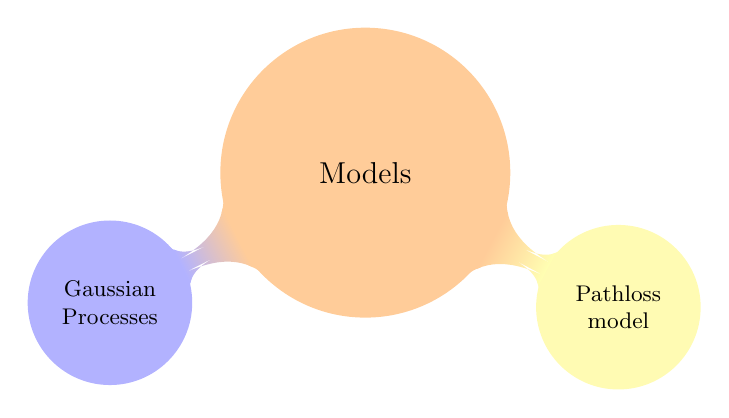
\begin{tikzpicture}[mindmap, grow cyclic, every node/.style=concept, concept color=orange!40,scale=0.91,transform shape,
	level 1/.append style={level distance=4cm,sibling angle=125}]
    \node{Models}[clockwise from=-28] 
    child [concept color=yellow!30]{ node (pmd) {Pathloss model}[clockwise from=-0]}
    child [concept color=blue!30]{ node (gp) {Gaussian Processes}[clockwise from=-260]}
    ;

\end{tikzpicture}
\caption{The two models used in the thesis.}
\end{figure}
\FloatBarrier

\begin{figure}[h!]
\centering
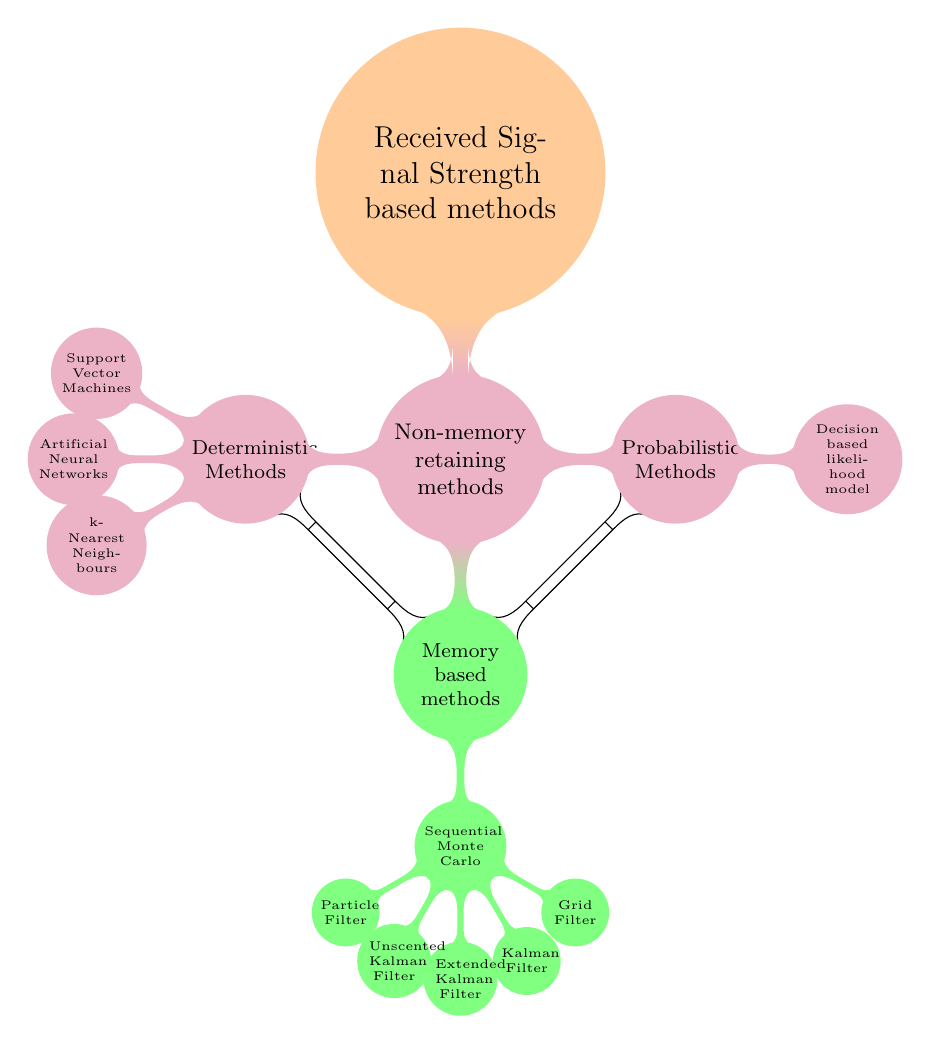
\begin{tikzpicture}[mindmap, grow cyclic, every node/.style=concept, concept color=orange!40,scale=0.91,transform shape,
	level 1/.append style={level distance=4cm,sibling angle=90},
    level 2/.append style={level distance=3cm,sibling angle=90}]
    
    \node{Received Signal Strength based methods}[clockwise from=-90] 
    
   child [concept color=purple!30] { node (nmem) {Non-memory retaining methods}[clockwise from=-0]
        child { node (pm) {Probabilistic Methods}[clockwise from=-0]
        		 child { node {Decision based likelihood model}}}
         child [concept color=green!50]{ node (mem) {Memory based methods}[clockwise from=-90]
        child { node {Sequential Monte Carlo}[clockwise from=-30]
        child { node {Grid Filter}}
         child { node {Kalman Filter}}
         child { node {Extended Kalman Filter}}
         child { node {Unscented Kalman Filter}}
         child{node {Particle Filter}}
        }}
        child { node (dm) {Deterministic Methods}[clockwise from=-150]
         child { node {k-Nearest Neighbours}}
         child { node {Artificial Neural Networks}}
         child { node {Support Vector Machines}}
         }
    };
    
    \begin{pgfonlayer}{background}
    \draw [circle connection bar]
       (mem) edge (dm)
       (pm) edge (mem);
  \end{pgfonlayer}
    



\end{tikzpicture}
\caption{The colorless edges denote that memory based methods can be used in conjunction with non-memory based methods.}
\end{figure}
\FloatBarrier

\section{Plan}


\subsection{Experiments:} 

\subsubsection{Data Analysis of RSSI values.} \label{exp-rssi}
\begin{enumerate}
\item Different Biases in RSSI measurements
\begin{itemize}
\item User's presence and without user's presence.
\item Different phones.
\item Different orientation of phones, angles, height? 
\item Different material of luminaires.(metal, plastic, metal+plastic). Its an added bonus if we can get the different luminaire material information from the BLE signal.
\item Different orientation of BT chip (cardinal directions and upwards and downwards)
\item Different calibration time for fingerprinting.
\item Different calibration points.
\item Fingerprint measuring while being still, only in 4 cardinal positions and while rotating.
\end{itemize}
\item With nearest node not working.
\item Experiment with different orientation of the mobile device. Hypothesis is that the there is 5 dBm difference for the change in orientation \cite{kaemar}.
\end{enumerate}

\subsubsection{Methods} 
Next, based on the results of the experiments above implement the methods described in the \ref{methods}.

\thiswillnotshow{
\section{Observations:}
\begin{enumerate}
\item The signal strengths from the nodes
\end{enumerate}}

\FloatBarrier
\begin{table}[H]
\centering
\caption{Plan for the thesis}
\label{tab-plan}
\begin{tabular}{|l|l|l|}
\hline
\textbf{Month}                   & \textbf{Task}                      & \textbf{Remarks}                                                                           \\ \hline
February                         & REST API                  & Completed                                                                         \\ \hline
\textbf{Meeting 1}               & Slides:     &  \url{https://goo.gl/Up9ejx}                                                                                 \\ \hline
March                            & Literature Review         & \shortstack[l]{1. Made extensive notes of the reading \\2. Will move it to thesis \\ 3. Made plan.} \\ \hline
                                 & \textbf{Phase 1}          &                                                                                   \\ \hline
April \& May                      & Get better model:       & Influence of various biases; Experiment in \ref{exp-rssi}                         \\ \hline
June: week 23, 24                & Buffer period for 2 weeks & End of Phase 1                                                                    \\ \hline
                                 & \textbf{Phase 2}          &                                                                                   \\ \hline
\shortstack[l]{June: week 25, 26\\July: week 27} & Methods                   & Non-memory based methods. As discussed in \ref{methods}:                          \\ \hline
\shortstack[l]{July: rest \\August}              & Methods                   & Memory based methods                                                              \\ \hline
                                 & \textbf{Phase 3}          &                                                                                   \\ \hline
September                        & Writing                   & Compile results, write it to thesis, and survey paper.                         \\ \hline
October & \\Novemeber            & Writing                   & Polish the thesis,comments from instructor and supervisors.                       \\ \hline
\end{tabular}
\end{table}


















%\begin{figure}
%\centering
%\includegraphics[width=0.3\textwidth]{frog.jpg}
%\caption{\label{fig:frog}This frog was uploaded via the project menu.}
%\end{figure}

\begin{thebibliography}{9}

\bibitem{fang}
Yeqing Fang, Zhongliang Deng, Chen Xue, Jichao Jiao, Hui Zeng, Ruoyu Zheng, Shunbao Lu, “\textit{Application of an Improved K Nearest Neighbor Algorithm in WiFi Indoor Positioning},” China Satellite Navigation Conference(CSNC), 2015 Proceedings: Volume III2015342, Berlin, Germany, Springer 517524, Lecture Notes in Electrical Engineering, 10.1007/978-3-662-46632-$2\_45$, doi:10.1155/2014/649276



\bibitem{yuan}
Xianghui Yuan, Feng Lian, and Chongzhao Han, “\textit{Models and Algorithms for Tracking Target with Coordinated Turn Motion},” Mathematical Problems in Engineering, vol. 2014, Article ID 649276, 10 pages, 2014. doi:10.1155/2014/649276

\bibitem{liu}
H. Liu, H. Darabi, P. Banerjee and J. Liu, “\textit{Survey of Wireless Indoor Positioning Techniques and Systems},” IEEE Transactions on Systems, Man, and Cybernetics, Part C (Applications and Reviews), vol. 37, number 6, 1067-1080 pages, Nov 2007, doi:10.1109/TSMCC.2007.905750

\bibitem{yiu}
Yiu, H. Darabi, P. Banerjee and J. Liu, “\textit{Locating User Equipment and Access Points using RSSI fingerprints},” IEEE Transactions on Systems, Man, and Cybernetics, Part C (Applications and Reviews), vol. 37, number 6, 1067-1080 pages, Nov 2007, doi:10.1109/TSMCC.2007.905750

\bibitem{kamath}
Arjun. P. Kamath,"\textit{Indoor Location-Based Services In The Telecommunications Network}", Master Thesis, Department of Communications and Networking, School of Electrical Engineering, Aalto University, 2014.

\bibitem{ferris}
B. Ferris, D. Fox, and N. Lawrence. WiFi SLAM Using Gaussian Process Latent Variable Model. In JCAI, January 2007.
 
\bibitem{kontact}
Beacon, link: https://store.kontakt.io/our-products/30-double-battery-beacon.html.
 
\bibitem{max}
Discussion with Max Bj\"orkgren on 9th March.
 
\bibitem{martin}
Martin Sauter (2010). "3.7.1 Mobility Management in the Cell-DCH State". From GSM to LTE: An Introduction to Mobile Networks and Mobile Broadband (eBook). John Wiley \& Sons. p. 160. ISBN 9780470978221.

\bibitem{geospatial}
 http://www.geospatialworld.net/wp-content/uploads/magazine/Geospatial-World-August-2014.pdf.

\bibitem{raivisto}
 Discussion with Tommi Raivisto on 16th March.

\bibitem{ble-ip-proj}
 Project done for the course CS-E4030 - Seminar on Gaussian processes, School of Science, Aalto University.
 
\bibitem{he}
Suining He, S.-H. Gary Chan. \textit{"Wi-Fi Fingerprint-based Indoor Positioning:Recent Advances and Comparisons"}, IEEE Communications Surveys and Tutorials, 2015.

\bibitem{kaemar}
Kaemarungsi et al, Analysis of WLAN’s received signal strength indication for indoor location fingerprinting,2011

\bibitem{richter}
Philipp Richter, Revisiting Gaussian Process Regression Modeling for Localization in Wireless Sensor Networks, 2015.
 
 \bibitem{honkavirta}
 Honkarvirta et al, 2009; Prasithsangaree et al, 2002
 
 \bibitem{deluca}
 De Luca et al, Performance evaluation of Indoor Localization Techniques Based on RF Power measurements from Active or Passive Devices.
 
\bibitem{hightower}
Hightower et al, Location Sensing Techniques, A Technical report, 2001

\bibitem{mazzullah}
Mazzullah Khan et al,2017

\bibitem{umar}
Umar Ahmad, iBeacon Localization, Master Thesis.

\bibitem{smailagic}
Smailagic et al, 2002

\bibitem{prasithsangaree}
Prasithsangaree et al, 2002

\bibitem{torres-sospedra}
Torres-Sospedra et al, A realistic evaluation of indoor positioning systems based on Wi-Fi fingerprinting, 2017

\bibitem{nurminen}
Nurminen et al, Particle Filter and smoother for Indoor localization,2013

\end{thebibliography}


\end{document}